\documentclass{standalone}
\usepackage{tikz}
\usetikzlibrary{patterns, positioning}


\begin{document}
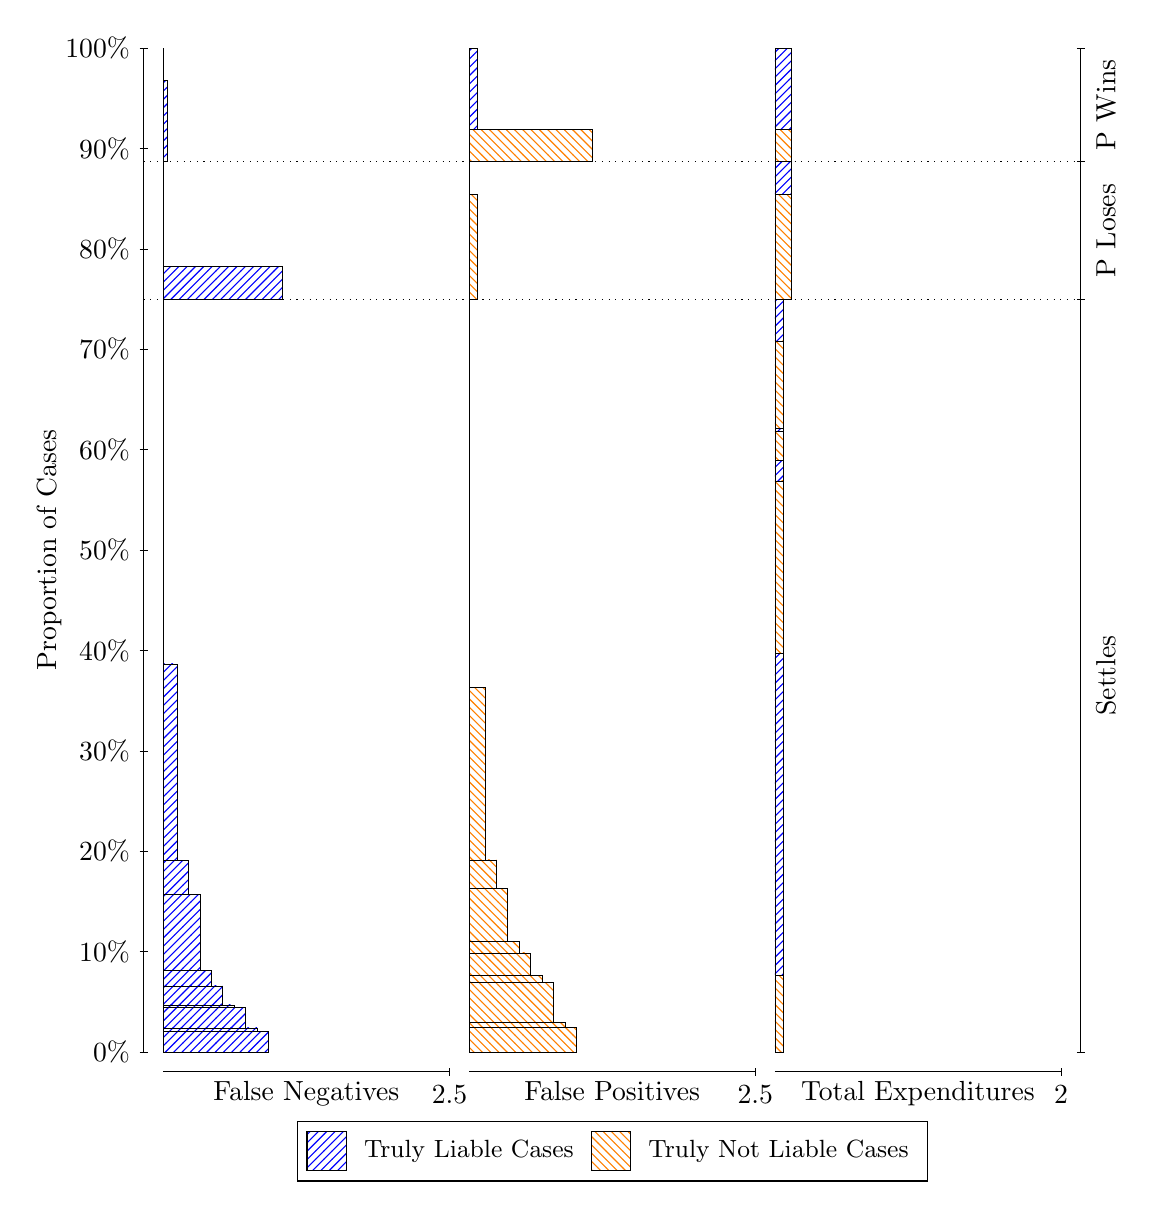
\begin{tikzpicture}
\draw[black, very thin] (1.5,1.75) -- (1.5,14.5);
\node[rotate=90, text=black, anchor=center] at (0.3, 8.125) {Proportion of Cases};
\draw[black, very thin] (1.45,1.75) -- (1.55,1.75);
\node[text=black, anchor=east] at (1.45, 1.75) {0\%};
\draw[black, very thin] (1.45,3.025) -- (1.55,3.025);
\node[text=black, anchor=east] at (1.45, 3.025) {10\%};
\draw[black, very thin] (1.45,4.3) -- (1.55,4.3);
\node[text=black, anchor=east] at (1.45, 4.3) {20\%};
\draw[black, very thin] (1.45,5.575) -- (1.55,5.575);
\node[text=black, anchor=east] at (1.45, 5.575) {30\%};
\draw[black, very thin] (1.45,6.85) -- (1.55,6.85);
\node[text=black, anchor=east] at (1.45, 6.85) {40\%};
\draw[black, very thin] (1.45,8.125) -- (1.55,8.125);
\node[text=black, anchor=east] at (1.45, 8.125) {50\%};
\draw[black, very thin] (1.45,9.4) -- (1.55,9.4);
\node[text=black, anchor=east] at (1.45, 9.4) {60\%};
\draw[black, very thin] (1.45,10.675) -- (1.55,10.675);
\node[text=black, anchor=east] at (1.45, 10.675) {70\%};
\draw[black, very thin] (1.45,11.95) -- (1.55,11.95);
\node[text=black, anchor=east] at (1.45, 11.95) {80\%};
\draw[black, very thin] (1.45,13.225) -- (1.55,13.225);
\node[text=black, anchor=east] at (1.45, 13.225) {90\%};
\draw[black, very thin] (1.45,14.5) -- (1.55,14.5);
\node[text=black, anchor=east] at (1.45, 14.5) {100\%};

\draw[black, very thin] (13.4,1.75) -- (13.4,14.5);
\draw[black, very thin] (13.35,1.75) -- (13.45,1.75);
\node[anchor=west] at (13.35, 1.75) {};
\draw[black, very thin] (13.35,11.311) -- (13.45,11.311);
\node[anchor=west] at (13.35, 11.311) {};
\draw[black, very thin] (13.35,13.056) -- (13.45,13.056);
\node[anchor=west] at (13.35, 13.056) {};
\draw[black, very thin] (13.35,14.5) -- (13.45,14.5);
\node[anchor=west] at (13.35, 14.5) {};

\draw[black, very thin, pattern color=blue, pattern=north east lines] (1.75,1.75) rectangle (3.0852,2.0116);
\draw[black, very thin, pattern color=blue, pattern=north east lines] (1.75,2.0116) rectangle (2.9399,2.0572);
\draw[black, very thin, pattern color=blue, pattern=north east lines] (1.75,2.0572) rectangle (2.7946,2.3117);
\draw[black, very thin, pattern color=blue, pattern=north east lines] (1.75,2.3117) rectangle (2.6492,2.3481);
\draw[black, very thin, pattern color=blue, pattern=north east lines] (1.75,2.3481) rectangle (2.5039,2.5882);
\draw[black, very thin, pattern color=blue, pattern=north east lines] (1.75,2.5882) rectangle (2.3586,2.7819);
\draw[black, very thin, pattern color=blue, pattern=north east lines] (1.75,2.7819) rectangle (2.2133,3.7481);
\draw[black, very thin, pattern color=blue, pattern=north east lines] (1.75,3.7481) rectangle (2.0679,4.1857);
\draw[black, very thin, pattern color=blue, pattern=north east lines] (1.75,4.1857) rectangle (1.9226,6.6797);
\draw[black, very thin, pattern color=orange, pattern=north west lines] (1.75,6.6797) rectangle (1.75,11.311);
\draw[black, very thin, pattern color=blue, pattern=north east lines] (1.75,11.311) rectangle (3.2578,11.722);
\draw[black, very thin, pattern color=orange, pattern=north west lines] (1.75,11.722) rectangle (1.75,13.056);
\draw[black, very thin, pattern color=blue, pattern=north east lines] (1.75,13.056) rectangle (1.8045,14.09);
\draw[black, very thin, pattern color=orange, pattern=north west lines] (1.75,14.09) rectangle (1.75,14.5);
\draw[black, very thin, pattern color=orange, pattern=north west lines] (5.6333,1.75) rectangle (6.9958,2.0594);
\draw[black, very thin, pattern color=orange, pattern=north west lines] (5.6333,2.0594) rectangle (6.8505,2.1231);
\draw[black, very thin, pattern color=orange, pattern=north west lines] (5.6333,2.1231) rectangle (6.7052,2.6294);
\draw[black, very thin, pattern color=orange, pattern=north west lines] (5.6333,2.6294) rectangle (6.5598,2.7178);
\draw[black, very thin, pattern color=orange, pattern=north west lines] (5.6333,2.7178) rectangle (6.4145,3.0095);
\draw[black, very thin, pattern color=orange, pattern=north west lines] (5.6333,3.0095) rectangle (6.2692,3.1534);
\draw[black, very thin, pattern color=orange, pattern=north west lines] (5.6333,3.1534) rectangle (6.1238,3.8233);
\draw[black, very thin, pattern color=orange, pattern=north west lines] (5.6333,3.8233) rectangle (5.9785,4.1889);
\draw[black, very thin, pattern color=orange, pattern=north west lines] (5.6333,4.1889) rectangle (5.8332,6.3811);
\draw[black, very thin, pattern color=blue, pattern=north east lines] (5.6333,6.3811) rectangle (5.6333,11.311);
\draw[black, very thin, pattern color=orange, pattern=north west lines] (5.6333,11.311) rectangle (5.7423,12.644);
\draw[black, very thin, pattern color=blue, pattern=north east lines] (5.6333,12.644) rectangle (5.6333,13.056);
\draw[black, very thin, pattern color=orange, pattern=north west lines] (5.6333,13.056) rectangle (7.1957,13.466);
\draw[black, very thin, pattern color=blue, pattern=north east lines] (5.6333,13.466) rectangle (5.7423,14.5);
\draw[black, very thin, pattern color=orange, pattern=north west lines] (9.5167,1.75) rectangle (9.6189,2.7178);
\draw[black, very thin, pattern color=blue, pattern=north east lines] (9.5167,2.7178) rectangle (9.6189,6.8093);
\draw[black, very thin, pattern color=orange, pattern=north west lines] (9.5167,6.8093) rectangle (9.6189,9.0015);
\draw[black, very thin, pattern color=blue, pattern=north east lines] (9.5167,9.0015) rectangle (9.6189,9.2631);
\draw[black, very thin, pattern color=orange, pattern=north west lines] (9.5167,9.2631) rectangle (9.6189,9.6287);
\draw[black, very thin, pattern color=blue, pattern=north east lines] (9.5167,9.6287) rectangle (9.6189,9.6743);
\draw[black, very thin, pattern color=orange, pattern=north west lines] (9.5167,9.6743) rectangle (9.6189,10.78);
\draw[black, very thin, pattern color=blue, pattern=north east lines] (9.5167,10.78) rectangle (9.6189,11.311);
\draw[black, very thin, pattern color=orange, pattern=north west lines] (9.5167,11.311) rectangle (9.721,12.644);
\draw[black, very thin, pattern color=blue, pattern=north east lines] (9.5167,12.644) rectangle (9.721,13.056);
\draw[black, very thin, pattern color=orange, pattern=north west lines] (9.5167,13.056) rectangle (9.721,13.466);
\draw[black, very thin, pattern color=blue, pattern=north east lines] (9.5167,13.466) rectangle (9.721,14.5);
\draw[black, dotted] (1.5,11.311) -- (13.4,11.311);
\draw[black, dotted] (1.5,13.056) -- (13.4,13.056);
\draw[black, very thin] (1.75,1.5) -- (5.3833,1.5);
\node[text=black, anchor=north] at (3.5667, 1.5) {False Negatives};
\draw[black, very thin] (5.3833,1.45) -- (5.3833,1.55);
\node[text=black, anchor=north] at (5.3833, 1.45) {2.5};

\draw[black, very thin] (5.6333,1.5) -- (9.2667,1.5);
\node[text=black, anchor=north] at (7.45, 1.5) {False Positives};
\draw[black, very thin] (9.2667,1.45) -- (9.2667,1.55);
\node[text=black, anchor=north] at (9.2667, 1.45) {2.5};

\draw[black, very thin] (9.5167,1.5) -- (13.15,1.5);
\node[text=black, anchor=north] at (11.333, 1.5) {Total Expenditures};
\draw[black, very thin] (13.15,1.45) -- (13.15,1.55);
\node[text=black, anchor=north] at (13.15, 1.45) {2};

\node[text=black, centered, rotate=90] at (13.72, 6.5304) {Settles};
\node[text=black, centered, rotate=90] at (13.72, 12.183) {P Loses};
\node[text=black, centered, rotate=90] at (13.72, 13.778) {P Wins};

\draw (7.449999999999999,1.5) node[draw=none] (baseCoordinate) {};
\begin{scope}[align=center]
        \matrix[scale=0.5, draw=black, below=0.5cm of baseCoordinate, nodes={draw}, column sep=0.1cm]{
            \node[rectangle, draw, minimum width=0.5cm, minimum height=0.5cm, pattern color=blue, pattern=north east lines] {}; &
            \node[draw=none, font=\small, text=black] (B) {Truly Liable Cases}; &
            \node[rectangle, draw, minimum width=0.5cm, minimum height=0.5cm, pattern color=orange, pattern=north west lines] {}; &
            \node[draw=none, font=\small, text=black] (B) {Truly Not Liable Cases}; \\
            };
\end{scope}

\end{tikzpicture}
\end{document}